\chapter{Arhitektura i dizajn sustava}

\noindent
Naš se sustav može podijeliti na tri podsustava:
\begin{description}
	\item[Web preglednik:] Lokalno instalirani program koji omogućuje prikaz sadržaja sa interneta. 
	Pomoću tog programa korisnik može poslati zahtjeve za 
	resursima ili poslati neke podatke web poslužitelju. Web preglednik, 
	nakon što dobije zatražene informacije od web poslužitelja, korisniku prikazuje sadržaj.

	\item[Web poslužitelj:] Centralni podsustav aplikacije koji obrađuje višestruke zahtjeve korisnika. Komunikaciju s klijentima ostvaruje preko
	HTTP protokola. Web poslužitelj može, na korisnički zahtjev, poslati datoteke ili primiti
	neke podatke koje može spremiti u bazu podataka.

	\item[Baza podataka:] Koristi se za pohranjivanje podataka web aplikacije. Sastavljena je od relacija koje
	predstavljaju entitete s određenim atributima koji su međusobno povezani definiranim
	odnosima. Web aplikacija često komunicira s bazom, povlačeći i davajući podatke bazi.
\end{description}

Klijent-server arhitektura uobičajen je način organizacije web aplikacija. U takvoj je arhitekturi sustav organiziran kao skup jednog ili više servisa koji mrežom komuniciraju s odgovarajućim klijentima. Glavna prednost ove arhitekture je to što distribuiranjem odgovornosti na više manjih servisa gradimo modularni sustav koji olakšava razvoj i otporniji je na greške; promjenom ili dodavanjem određenog servisa ne utječemo na ostatak sustava. Iako u našoj implementaciji ne iskorištavamo sve prednosti ove arhitekture jer nam je potreban samo jedan server (servis za pristup bazi podataka, backend) i jedan programski klijent (sustav za prikazivanje podataka u web pregledniku, frontend), odvajanje odgovornosti znatno nam je olakšalo razvoj aplikacije.

Servis za pristup bazi podataka razvijen je u Pythonu, koristeći programski mikrookvir Flask. U svojoj osnovi Flask je znatno manji od sličnih okvira (Django, FastAPI) te pruža lakši i brži razvoj uz sve potrebne funkcionalnosti za razvoj HTTP programskog sučelja. Od dostupnih ORM-ova, Flask se najbolje može integrirati sa SqlAlchemyjem pa je on korišten za spajanje na PostgreSQL bazu podataka, stvaranje i izvršavanje upita te upravljanje preslikavanjem relacija iz baze u Python objekte. Za serijalizaciju objekata iz baze (posebice prilikom oblikovanja HTTP odgovora) korišten je Marshmallow kao vrlo malena i učinkovita biblioteka.

Web sučelje aplikacije razvijeno je u okruženju React, a pokreće ga Node.js. Razvijen u Meti, React je Javascript biblioteka za izgradnju korisničkih sučelja kompozicijom komponenti pomoću kojih se optimizira proces prikazivanja i osvježavanja sučelja. S velikom zajednicom koja ga koristi i razvija te iznimno kvalitetnom podrškom React je bio najpouzdaniji odabir za tehnologiju za razvoj frontenda. U razvoju smo koristili Typescript kao pouzdaniju inačicu Javascripta u smislu izbjegavanja logičkih pogreški prilikom razvoja strogom i statičkom provjerom tipova podataka.

Kako bismo centralizirali pohranjivanje stanja aplikacije i odvojili logiku upravljanja tim stanjem od logike izgradnje komponenti, uz React koristili smo i Redux. Uvođenjem Reduxa, MVC arhitektura nametnula se kao intuitivan način za organizaciju logike prikazivanja podataka korisniku. Naime, iako se određene funkcionalnosti Reacta mogu koristiti za pohranjivanje stanja aplikacije i upravljanje njime, korištenjem samo Reacta otežali smo razvoj i skaliranje aplikacije. Tako se u našoj implementaciji stanje aplikacije pohranjuje u Reduxovom storeu (model), prikazuje se korisniku preko sučelja napravljenog u Reactu (view), a osvježavanje ili mijenjanje prikazanih podataka odgovornost je Reduxovih reducera (controller).

		\section{Baza podataka}

		Naš sustav koristi bazu podataka koja se temelji na relacijskom modelu podataka i koristi tablice (relacije) za organizaciju i pohranu podataka. Entiteti naše baze su: 
		\begin{itemize}
			\item Jezik
			\item Rječnik
			\item Riječ
			\item Korisnik
			\item Fraza
			\item Posuda
		\end{itemize}
		
			\subsection{Opis tablica}
			

				\textbf{Korisnik} Entitet Korisnik sadrži sve informacije o korisniku. Atributi korisnika su: userId(primarni ključ), ime, prezime, email, lozinka, korisnikStvorenNa, uloga i promijenioLozinku. Korisnik je u \textit{Many-To-One} vezi s tablicom StanjeRiječi.
				
				
				\begin{longtblr}[
					label=none,
					entry=none
					]{
						width = \textwidth,
						colspec={|X[15,l]|X[6, l]|X[20, l]|}, 
						rowhead = 1,
					} %definicija širine tablice, širine stupaca, poravnanje i broja redaka naslova tablice
					\hline \SetCell[c=3]{c}{\textbf{Korisnik}}	 \\ \hline[3pt]
					\SetCell{LightGreen}userId & INT & Identifikacijski ključ korisnika
					  	\\ \hline
					ime	& VARCHAR & Korisnikovo ime  	\\ \hline 
					prezime & VARCHAR & Korisnikovo prezime \\ \hline
					email & VARCHAR & Korisnikov email\\ \hline 
					lozinka & VARCHAR & Korisnikova lozinka \\ \hline
					korisnikStvorenNa & DATETIME & Datum stvaranja računa \\ \hline
					uloga & VARCHAR & Korisnikova uloga (učenik ili admin) \\ \hline
					promijenioLozinku & BOOLEAN & Oznaka je li korisnik promijenio lozinku \\ \hline
					
				\end{longtblr}
				
				\textbf{Rječnik} Entitet Rječnik sadrži sve informacije o rječniku. Njegovi atributi su su: rječnikId(primarni ključ), nazivRječnik, rječnikStvorenNa i jezikId. Rječnik je u \textit{Many-To-One} vezi s tablicom RječnikRiječi te je u \textit{Many-To-One} vezi s entitetom Jezik.


				\begin{longtblr}[
					label=none,
					entry=none
					]{
						width = \textwidth,
						colspec={|X[15,l]|X[6, l]|X[20, l]|}, 
						rowhead = 1,
					} %definicija širine tablice, širine stupaca, poravnanje i broja redaka naslova tablice
					\hline \SetCell[c=3]{c}{\textbf{Rječnik}}	 \\ \hline[3pt]
					\SetCell{LightGreen}rječnikId & INT & Identifikacijski ključ rječnika
					  	\\ \hline
					nazivRječnik	& VARCHAR & Naziv rječnika  	\\ \hline 
					rječnikStvorenNa & DATE & Datum stvaranja rječnika \\ \hline
					\SetCell{LightBlue}
					jezikId & INT & Identifikacijski ključ jezika rječnika\\ \hline 
					
				\end{longtblr}

				\textbf{Riječ} Entitet Riječ sadrži sve informacije o riječi u sustavu. Njeni atributi su su: riječId(primarni ključ), hrvNaziv, straniNaziv, audioPath i jezikId. Entitet Riječ je u \textit{Many-To-One} vezi s entitetom Jezik, u \textit{Many-To-One} vezi s tablicom RiječRječnik, u \textit{One-To-Many} vezi s entitetom Fraza te u \textit{Many-To-One} vezi s tablicom StanjeRiječi.

				\begin{longtblr}[
					label=none,
					entry=none
					]{
						width = \textwidth,
						colspec={|X[15,l]|X[6, l]|X[20, l]|}, 
						rowhead = 1,
					} %definicija širine tablice, širine stupaca, poravnanje i broja redaka naslova tablice
					\hline \SetCell[c=3]{c}{\textbf{Riječ}}	 \\ \hline[3pt]
					\SetCell{LightGreen}riječId & INT & Identifikacijski ključ riječi
					  	\\ \hline
					hrvNaziv & VARCHAR & Naziv riječi na hrvatskom \\ \hline
					straniNaziv	& VARCHAR & Naziv rječi na stranom jeziku 	\\ \hline 
					audioPath	& VARCHAR & Put do audio datoteke s izgovorom riječi  	\\ \hline 
					\SetCell{LightBlue}
					jezikId & INT & Identifikacijski ključ jezika rječnika\\ \hline 
					
				\end{longtblr}

				\textbf{Jezik} Entitet Jezik sadrži sve informacije o nekom jeziku u sustavu. Njegovi atributi su su: jezikId(primarni ključ), nazivJezik i isoOznaka. Entitet Jezik je u \textit{One-To-Many} vezi s entitetom Rječnik te u \textit{One-To-Many} vezi s entitetom Riječ.


				\begin{longtblr}[
					label=none,
					entry=none
					]{
						width = \textwidth,
						colspec={|X[15,l]|X[6, l]|X[20, l]|}, 
						rowhead = 1,
					} %definicija širine tablice, širine stupaca, poravnanje i broja redaka naslova tablice
					\hline \SetCell[c=3]{c}{\textbf{Jezik}}	 \\ \hline[3pt]
					\SetCell{LightGreen}jezikId & INT & Identifikacijski ključ jezika
					  	\\ \hline
					nazivJezik & VARCHAR & Naziv jezika \\ \hline
					isoOznaka	& CHAR(2) & ISO oznaka jezika 	\\ \hline 
					 
					
				\end{longtblr}

				\textbf{Fraza} Entitet Fraza sadrži sve informacije o nekoj frazi u sustavu. Njeni atributi su su: frazaId(primarni ključ), fraza i riječId. Entitet Fraza je u \textit{Many-To-One} vezi s entitetom Riječ.


				\begin{longtblr}[
					label=none,
					entry=none
					]{
						width = \textwidth,
						colspec={|X[15,l]|X[6, l]|X[20, l]|}, 
						rowhead = 1,
					} %definicija širine tablice, širine stupaca, poravnanje i broja redaka naslova tablice
					\hline \SetCell[c=3]{c}{\textbf{Fraza}}	 \\ \hline[3pt]
					\SetCell{LightGreen}frazaId & INT & Identifikacijski ključ fraze
					  	\\ \hline
					fraza & VARCHAR & Puna fraza \\ \hline
					\SetCell{LightBlue}riječId & INT & Identifikacijski ključ riječi iz fraze
					  	\\ \hline
					 
					
				\end{longtblr}

				\textbf{RiječRječnik} Tablica RiječRječnik povezuje sve riječi s pripadnim rječnikom. Njeni atributi su su: riječId(primarni ključ) te rječnikId(primarni ključ). Tablica RiječRječnik je u \textit{One-To-Many} vezi s entitetom Riječ i u \textit{One-To-Many} vezi s entitetom Rječnik.

				\begin{longtblr}[
					label=none,
					entry=none
					]{
						width = \textwidth,
						colspec={|X[15,l]|X[6, l]|X[20, l]|}, 
						rowhead = 1,
					} %definicija širine tablice, širine stupaca, poravnanje i broja redaka naslova tablice
					\hline \SetCell[c=3]{c}{\textbf{RiječRječnik}}	 \\ \hline[3pt]
					\SetCell{LightGreen}riječId & INT & Identifikacijski ključ riječi
					  	\\ \hline
					\SetCell{LightGreen}rječnikId & INT &Identifikacijski ključ rječnika
					\\ \hline
					 
					
				\end{longtblr}


				\textbf{StanjeRiječi} Tablica StanjeRiječi povezuje korisnika s riječima i njima pripadnim "posudama". Njeni atributi su su: userId(primarniKljuč), riječId(primarniKljuč) i posudaId. Tablica StanjeRiječi je u \textit{One-To-Many} vezi s entitetom Riječ, u \textit{One-To-Many} vezi s entitetom Korisnik te u \textit{One-To-One} vezi s entitetom Posuda.

				\begin{longtblr}[
					label=none,
					entry=none
					]{
						width = \textwidth,
						colspec={|X[15,l]|X[6, l]|X[20, l]|}, 
						rowhead = 1,
					} %definicija širine tablice, širine stupaca, poravnanje i broja redaka naslova tablice
					\hline \SetCell[c=3]{c}{\textbf{StanjeRiječi}}	 \\ \hline[3pt]
					\\ \hline[3pt]
					\SetCell{LightGreen}userId & INT & Identifikacijski ključ korisnika
					  	\\ \hline
					\SetCell{LightGreen}riječId & INT & Identifikacijski ključ riječi
					  	\\ \hline
					\SetCell{LightBlue}posudaId & INT & Identifikacijski ključ posude
					  	\\ \hline 
					
				\end{longtblr}

				\textbf{Posuda} Entitet Posuda predstavlja sve posude i njihove intervale. Njeni atributi su su: posudaId(primarni ključ) i interval. Tablica Posuda je u \textit{One-To-One} vezi s tablicom StanjeRiječi.


				\begin{longtblr}[
					label=none,
					entry=none
					]{
						width = \textwidth,
						colspec={|X[15,l]|X[6, l]|X[20, l]|}, 
						rowhead = 1,
					} %definicija širine tablice, širine stupaca, poravnanje i broja redaka naslova tablice
					\hline \SetCell[c=3]{c}{\textbf{Posuda}}	 \\ \hline[3pt]
					\SetCell{LightGreen}posudaId & INT & Identifikacijski ključ posude
					  	\\ \hline
					interval & INT & Interval čekanja do ponovnog pojavljivanja riječi \\ \hline
					
					 
					
				\end{longtblr}

\eject
			
			\subsection{Dijagram baze podataka}	
			
			\begin{figure}[htp]
				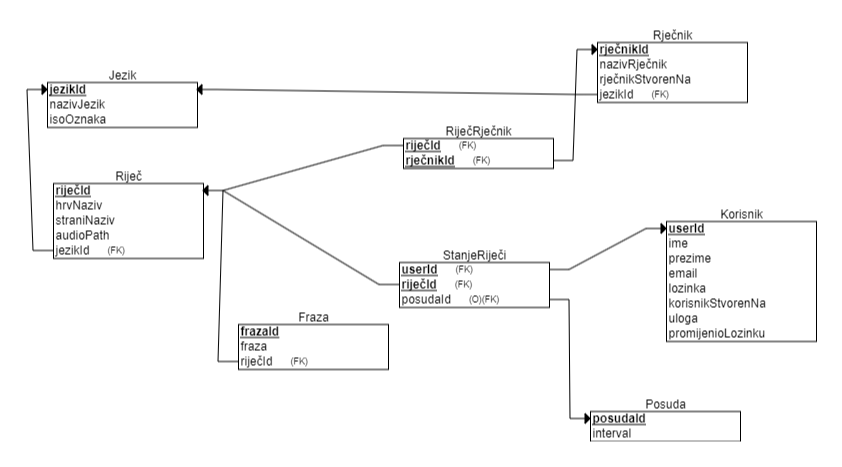
\includegraphics[scale=0.5]{dijagrami/relacijski_model.png}
				\centering
				\caption{Relacijska shema baze podataka}
				\label{fig:dijagram_REL-SH_BP}
			\end{figure}

				\begin{figure}[htp]
					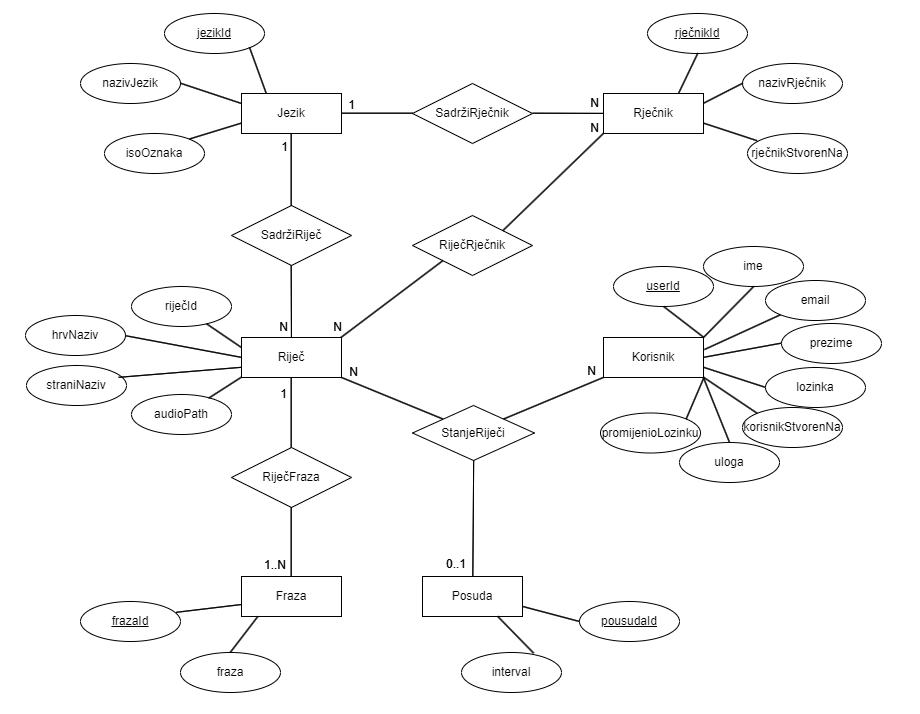
\includegraphics[scale=0.5]{dijagrami/ER_model_BP_3.png}
					\centering
					\caption{ER model baze podataka}
					\label{fig:dijagram_ER-BP}
				\end{figure}
			
			\eject
			
			
		\section{Dijagram razreda}
		
\subsection{Razredi na backendu}

Ova se skupina razreda (Slika \ref{fig:class-back}) izravno preslikava u bazu podataka tako da se za svaki razred stvara jedna tablica u bazi. Dakle, svi su razredi svedeni na treću normalnu formu i ni u kojem slučaju ne mogu biti povezani pridruživanjem (agregacijom ili asocijacijom). U generičkim funkcionalnostima implementiran je razred Korisnik.

\subsubsection{db.Model}

Razred koj dolazi iz SqlAlchemyja koji koristimo u pozadini za komunikaciju s 
bazom podataka. Ovaj razred nasljeđuju svi razredi u skupini modela na backendu zato što on
pruža potrebne funkcionalnosti za slanje i povlačenje podataka u bazu.


\subsubsection{Razred Jezik}

Služi za modeliranje jezika te je opisan atributima identifikatora,
naziva jezika i iso oznake. Atributi su privatni, te ima javni konstruktor.

\subsubsection{Razred Riječ}

Služi za modeliranje riječi, najmanje jedinice učenja u aplikaciji.
Razred sadrži atribute: identifikator riječi, hrvatski naziv, strani naziv,
putanju na audiodatoteku izgovora riječi na stranom jeziku i identifikator jezika
na kojem su audiozapis i strani naziv. Atributi su privatni i ima javni konstruktor.

\subsubsection{Razred Rječnik}

Služi za modeliranje rječnika, tj. kolekcije riječi. Razred je opisan atributima identifikatora, naziva rječnika, datuma njegovog stvorenja i jezika riječi koje sadrži. Atributi su privatni te ima javni konstruktor.

\subsubsection{Razred StanjeRiječi}

Služi kao razred koji prati stanje riječi, tj. je li riječ naučena. Opisan je s atributima: identifikatora korisnika, identifikatora riječi i identifikatora posude. Atributi su privatni i ima javni konstruktor.

\subsubsection{Razred Posuda}

Služi za modeliranje posude, opisan sa identifikatorom posude i intervalom.
Atributi su privatni i ima javni konstruktor.

\subsubsection{Razred Fraza}

Služi za modeliranje fraze koja prati riječ na stranom jeziku za lakše
učenje konteksta. Razred je opisan s atributima identifikatora fraze, samom frazom i identifikatorom riječi uz koju je fraza povezana. Atributi su privatni i ima javni konstruktor.


\subsubsection{Razred Korisnik}

Služi za modeliranje korisnika. Baza podataka razlikuje administratore i učenike po njihovoj ulozi,
ne smatra ih različitim entitetima. Razred opisuju atributi identifikatora korisnika, imena, prezimena,
adrese elektroničke pošte, lozinke za račun, trenutka stvaranja korisnika, uloge i zastavice
koja provjerava promjenu lozinke. Atributi su privatni i razred ima javni konstruktor.

\begin{figure}[H]
	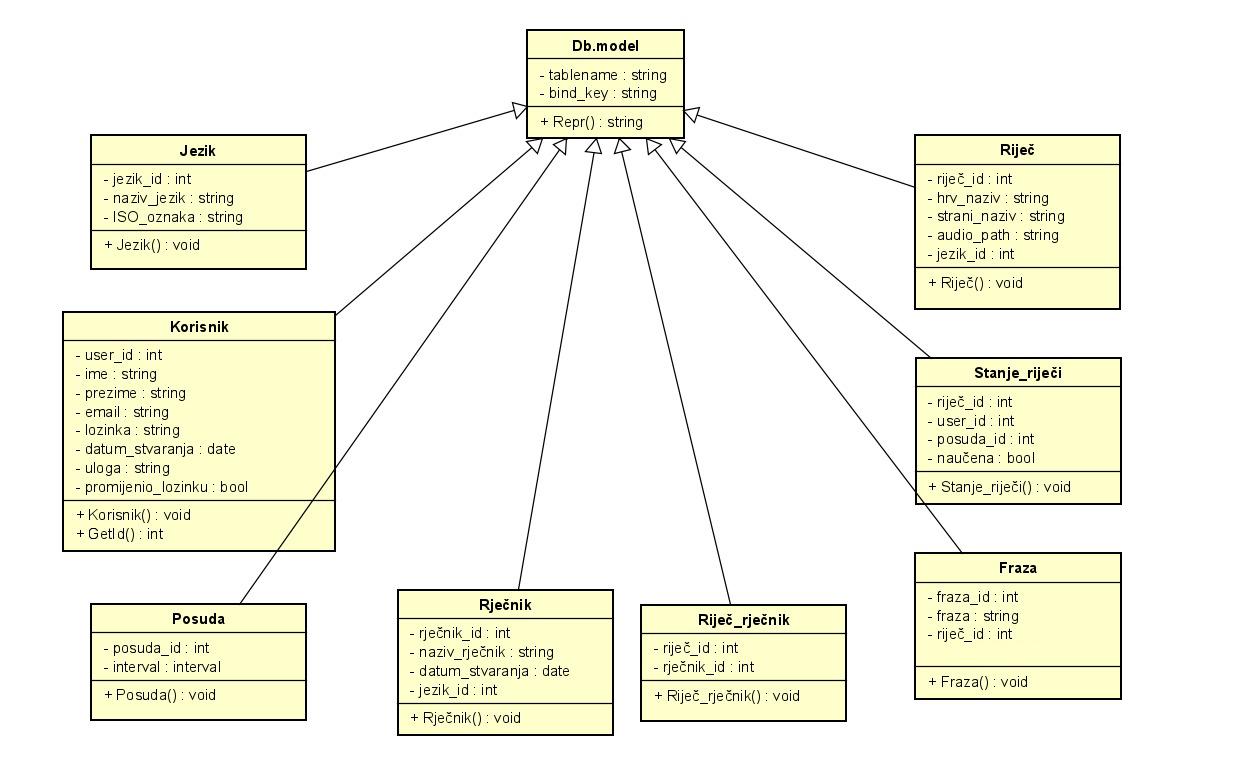
\includegraphics[scale=0.35]{dijagrami/class_back.jpeg}
	\centering
	\caption{Dijagram razreda za backend dio aplikacije}
	\label{fig:class-back}
\end{figure}

\subsection{Razredi na frontendu}

Razredi na frontend dijelu aplikacije podijeljeni su u tri skupine. Isječke (slices) u kojima se spremaju podaci tipa Models, a čije metode primaju podatke iz Inputs skupine razreda. Kako su isječci međusobno neovisni i radi preglednosti razredi na klijentskom dijelu aplikacije prikazani su u nekoliko dijagrama, ovisno o isječku s kojim su povezani.
\begin{description}
	\item[Modeli] su reprezentacije entiteta s backend dijela aplikacije. Backend modeli ne preslikavaju se izravno u odgovarajuće frontend modele, već se proširuju s dodatnim podacima iz povezanih tablica. Tako, primjerice, dok razredi Riječ i Fraza na backendu nisu povezani, razred Riječ na frontendu u sebi ima listu objekata razreda Fraza.
	\item[Input] razredi predstavljaju \textit{data transfer} objekte. Objekti tog razreda izravno se mogu pohraniti u tijelo HTTP zahtjeva i odgovaraju onoj strukturi u kojoj  pojedina pristupna točka na backendu očekuje primiti podatke.
	\item[Slice] razredi specifični su za implementiranu arhitekturu koja koristi Redux za upravljanje stanjem aplikacije. S ciljem odvajanja odgovornosti, stanje cijele aplikacije podijeljeno je na proizvoljan broj samostalnih cjelina (isječak, \textit{slice}) koje upravljaju i pohranjuju podatke iz isključivo jedne domene. Stanje u određenom isječku može se mijenjati samo preko njegovih metoda, a unutar njih se nerijetko pozivaju \textit{axios} metode za slanje HTTP zahtjeva backend dijelu aplikacije jer se rezultati tih poziva moraju spremati upravo u stanje aplikacije. Ukupno je implementirano sedam razreda za isječke stanja:
	
	\begin{packed_enum}

		\item \emph{Admin} -- upravljanje administratorima
		\item \emph{Auth} -- podaci o trenutno prijavljenom korisniku
		\item \emph{Dictionaries} -- upravljanje rječnicima 
		\item \emph{Language} -- dostupni jezici i trenutno odabran jezik
		\item \emph{Student Dictionaries} -- rječnici nekog jezika s dodatnim podacima koji se prikazuju učeniku
		\item \emph{Study Session} -- podaci potrebni za učenje u bilo kojem načinu učenja
		\item \emph{Words} -- upravljanje riječima
		
	\end{packed_enum}
	
\end{description}

\begin{figure}[htp]
	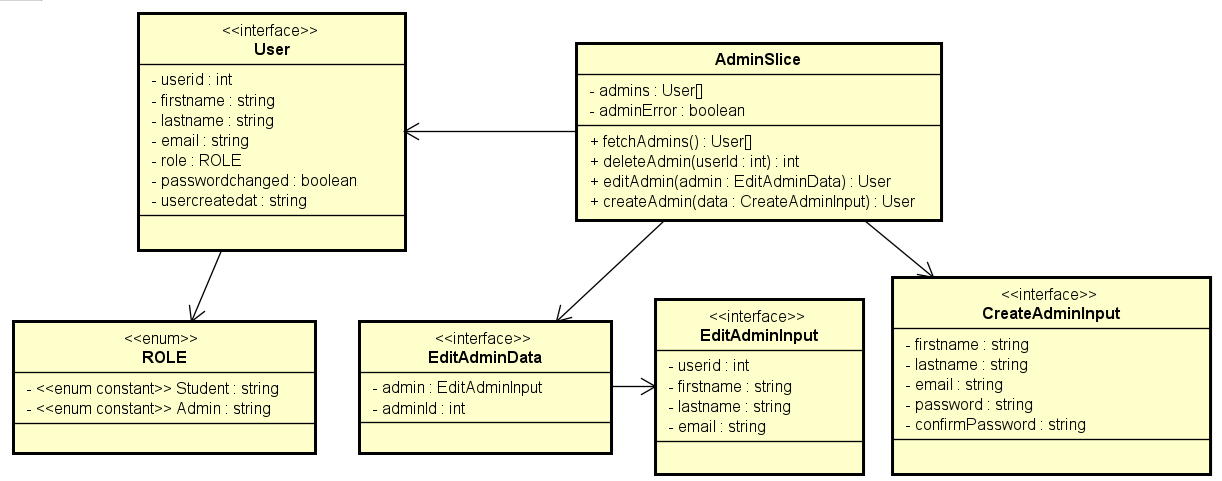
\includegraphics[scale=0.47]{dijagrami/AdminSlice.png}
	\centering
	\caption{Dijagram razreda za slice Admin}
	\label{fig:cls-admin}
\end{figure}

\begin{figure}[htp]
	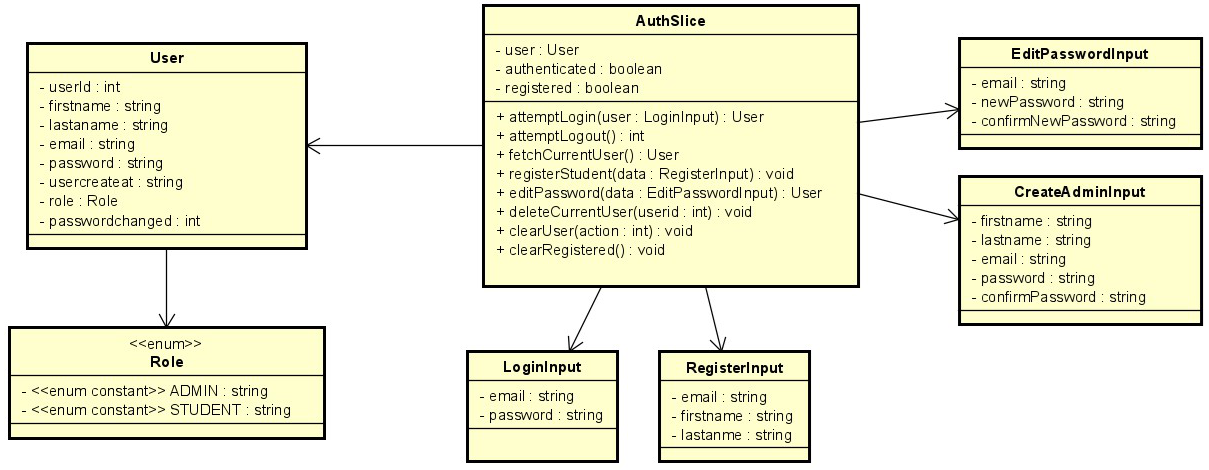
\includegraphics[scale=0.6]{dijagrami/authSlice.png}
	\centering
	\caption{Dijagram razreda za slice Auth}
	\label{fig:cls-auth}
\end{figure}

\begin{figure}[htp]
	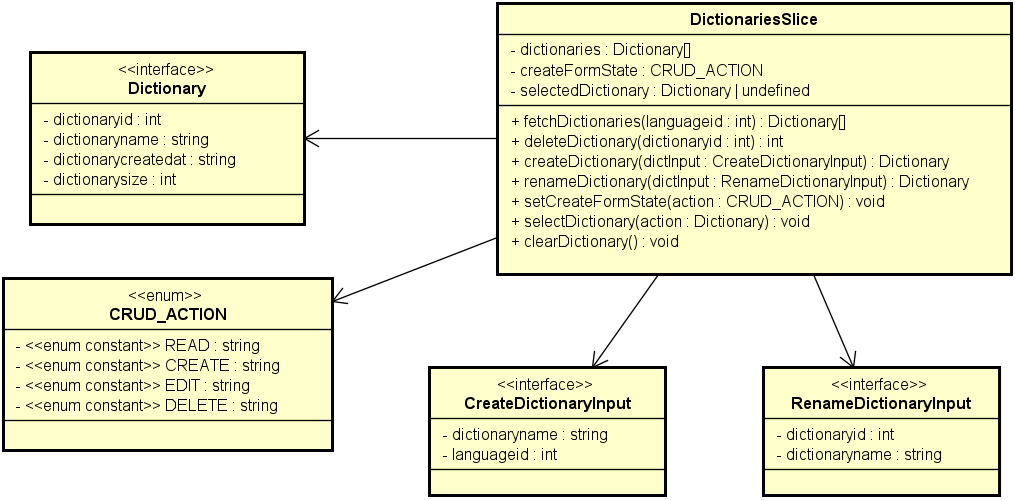
\includegraphics[scale=0.57]{dijagrami/DictionariesSlice.png}
	\centering
	\caption{Dijagram razreda za slice Dictionaries}
	\label{fig:cls-dict}
\end{figure}

\begin{figure}[htp]
	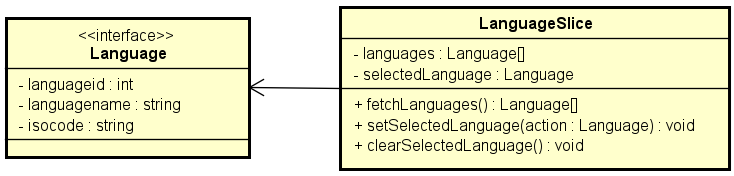
\includegraphics[scale=0.6]{dijagrami/LanguageSlice.png}
	\centering
	\caption{Dijagram razreda za slice Language}
	\label{fig:cls-lang}
\end{figure}

\begin{figure}[htp]
	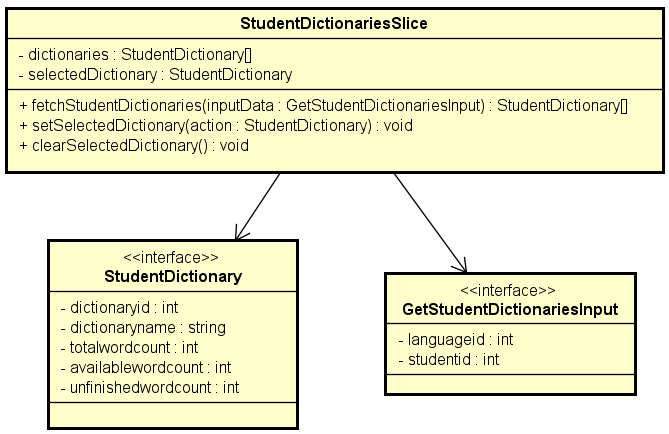
\includegraphics[scale=0.6]{dijagrami/StudentDictionariesSlice.png}
	\centering
	\caption{Dijagram razreda za slice Student Dictionaries}
	\label{fig:cls-student-dict}
\end{figure}

\begin{figure}[htp]
	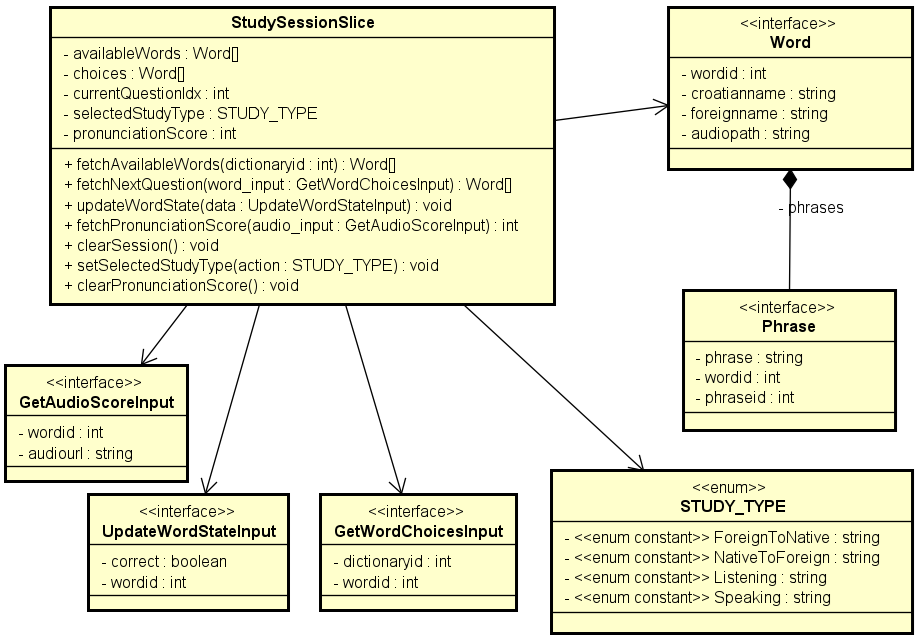
\includegraphics[scale=0.5]{dijagrami/StudySessionSlice.png}
	\centering
	\caption{Dijagram razreda za slice Study Session}
	\label{fig:cls-study-sesion}
\end{figure}

\begin{figure}[htp]
	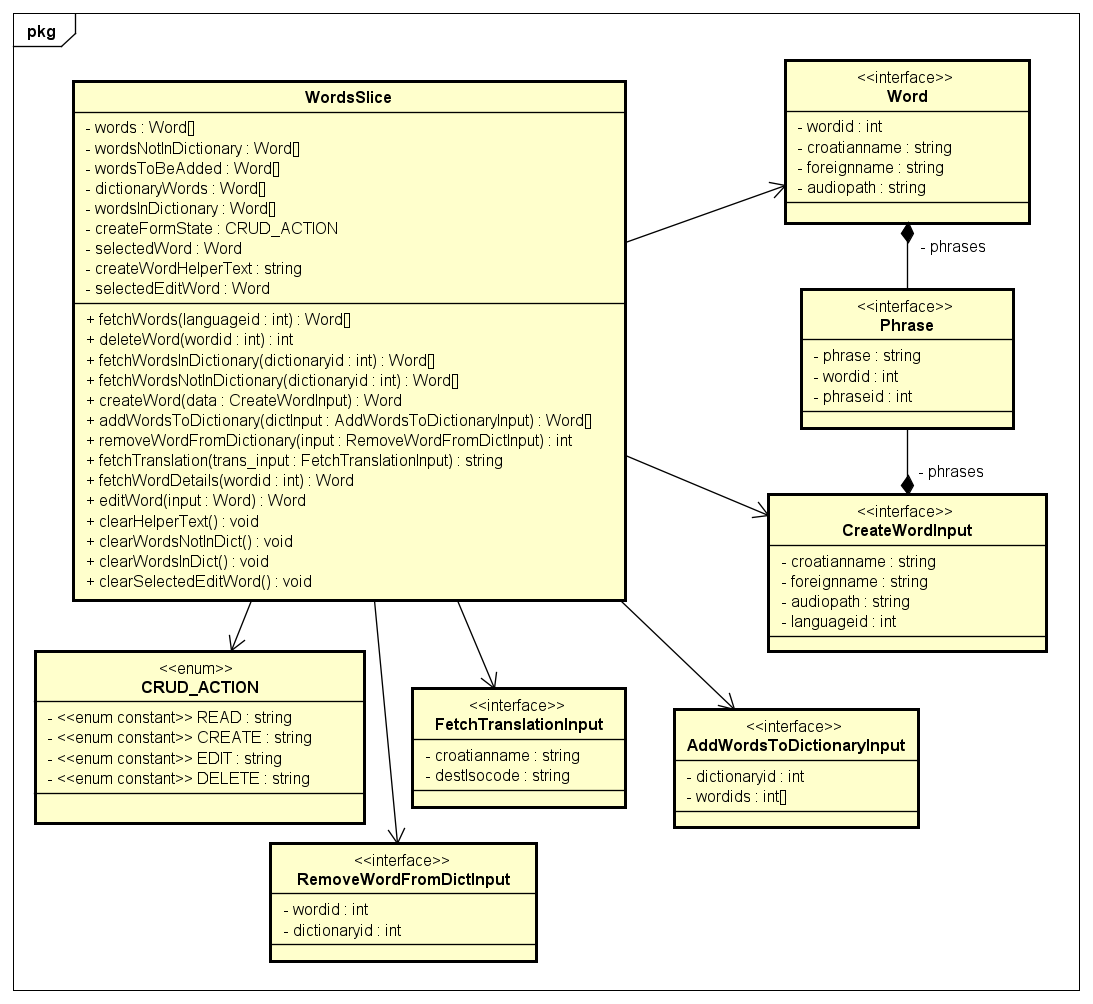
\includegraphics[scale=0.5]{dijagrami/WordsSlice.png}
	\centering
	\caption{Dijagram razreda za slice Words}
	\label{fig:cls-words}
\end{figure}

\eject


		\section{Dijagram stanja}
			
			
\begin{figure}[htp]
	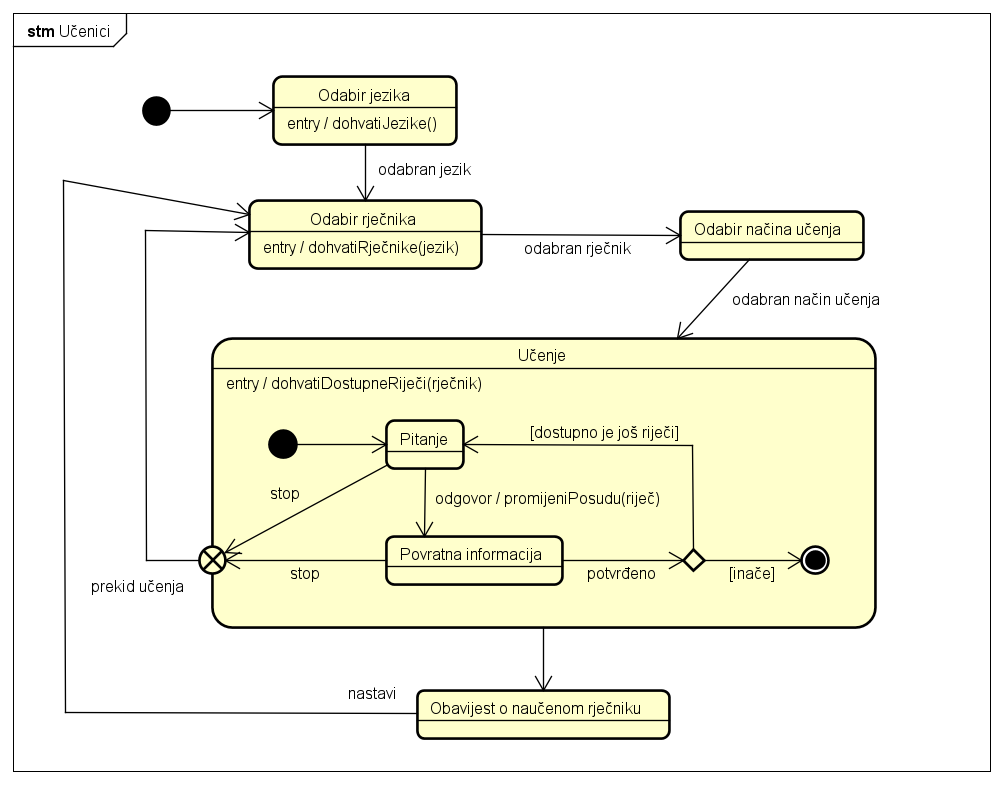
\includegraphics[scale=0.5]{dijagrami/state_ucenici.png}
	\centering
	\caption{Dijagram stanja - sučelje za učenike}
	\label{fig:state-ucenici}
\end{figure}

\begin{figure}[htp]
	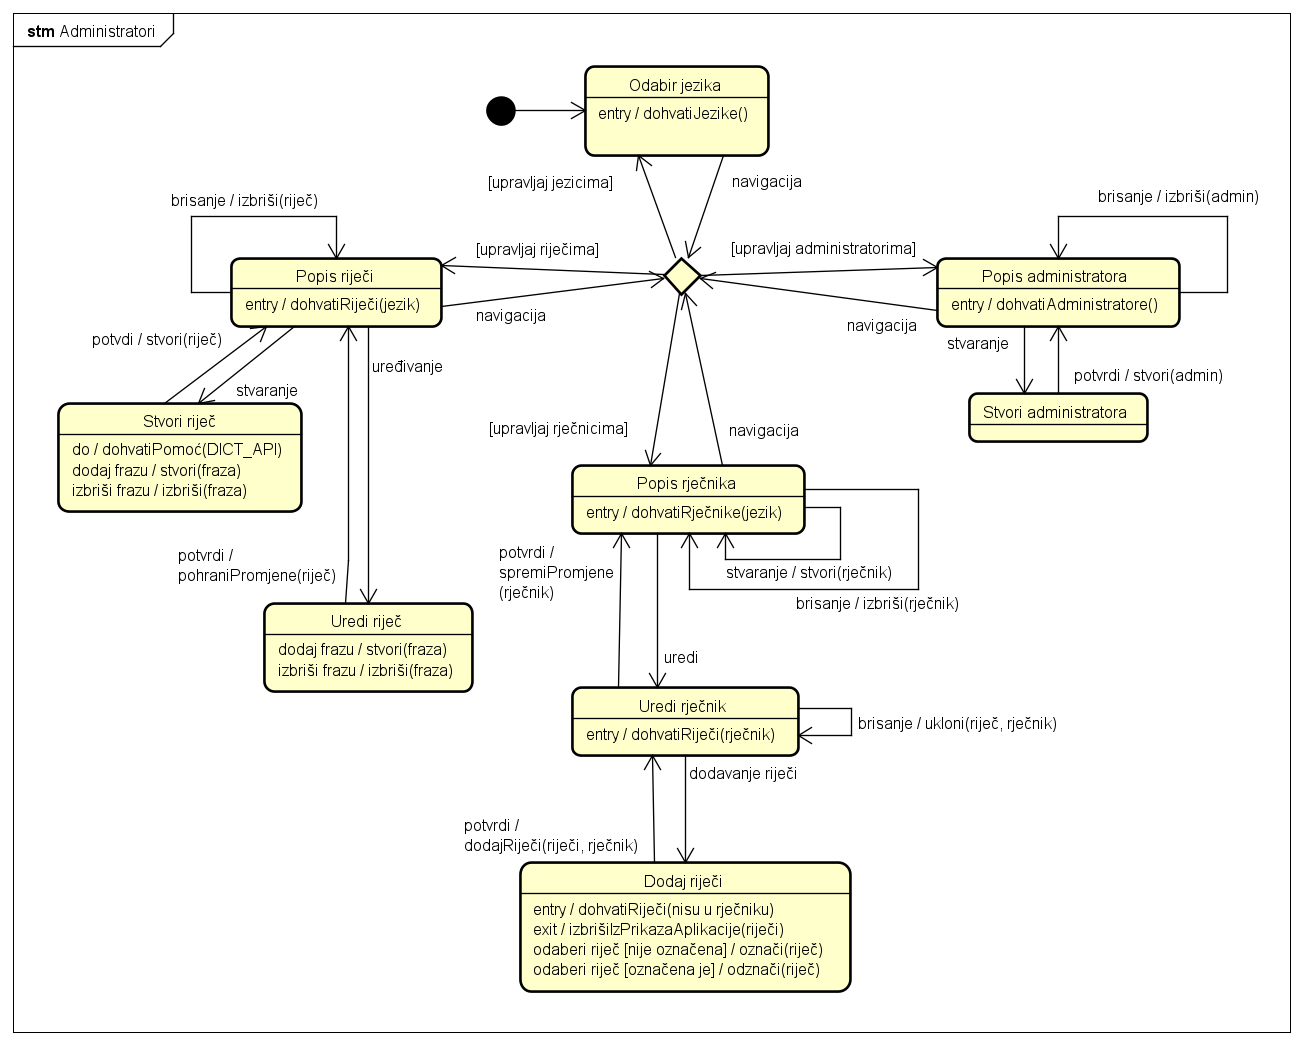
\includegraphics[scale=0.4]{dijagrami/state_administratori.png}
	\centering
	\caption{Dijagram stanja - sučelje za administratore}
	\label{fig:state-admin}
\end{figure}
			
			
			\eject 
		
		\section{Dijagram aktivnosti}
			
\begin{figure}[htp]
	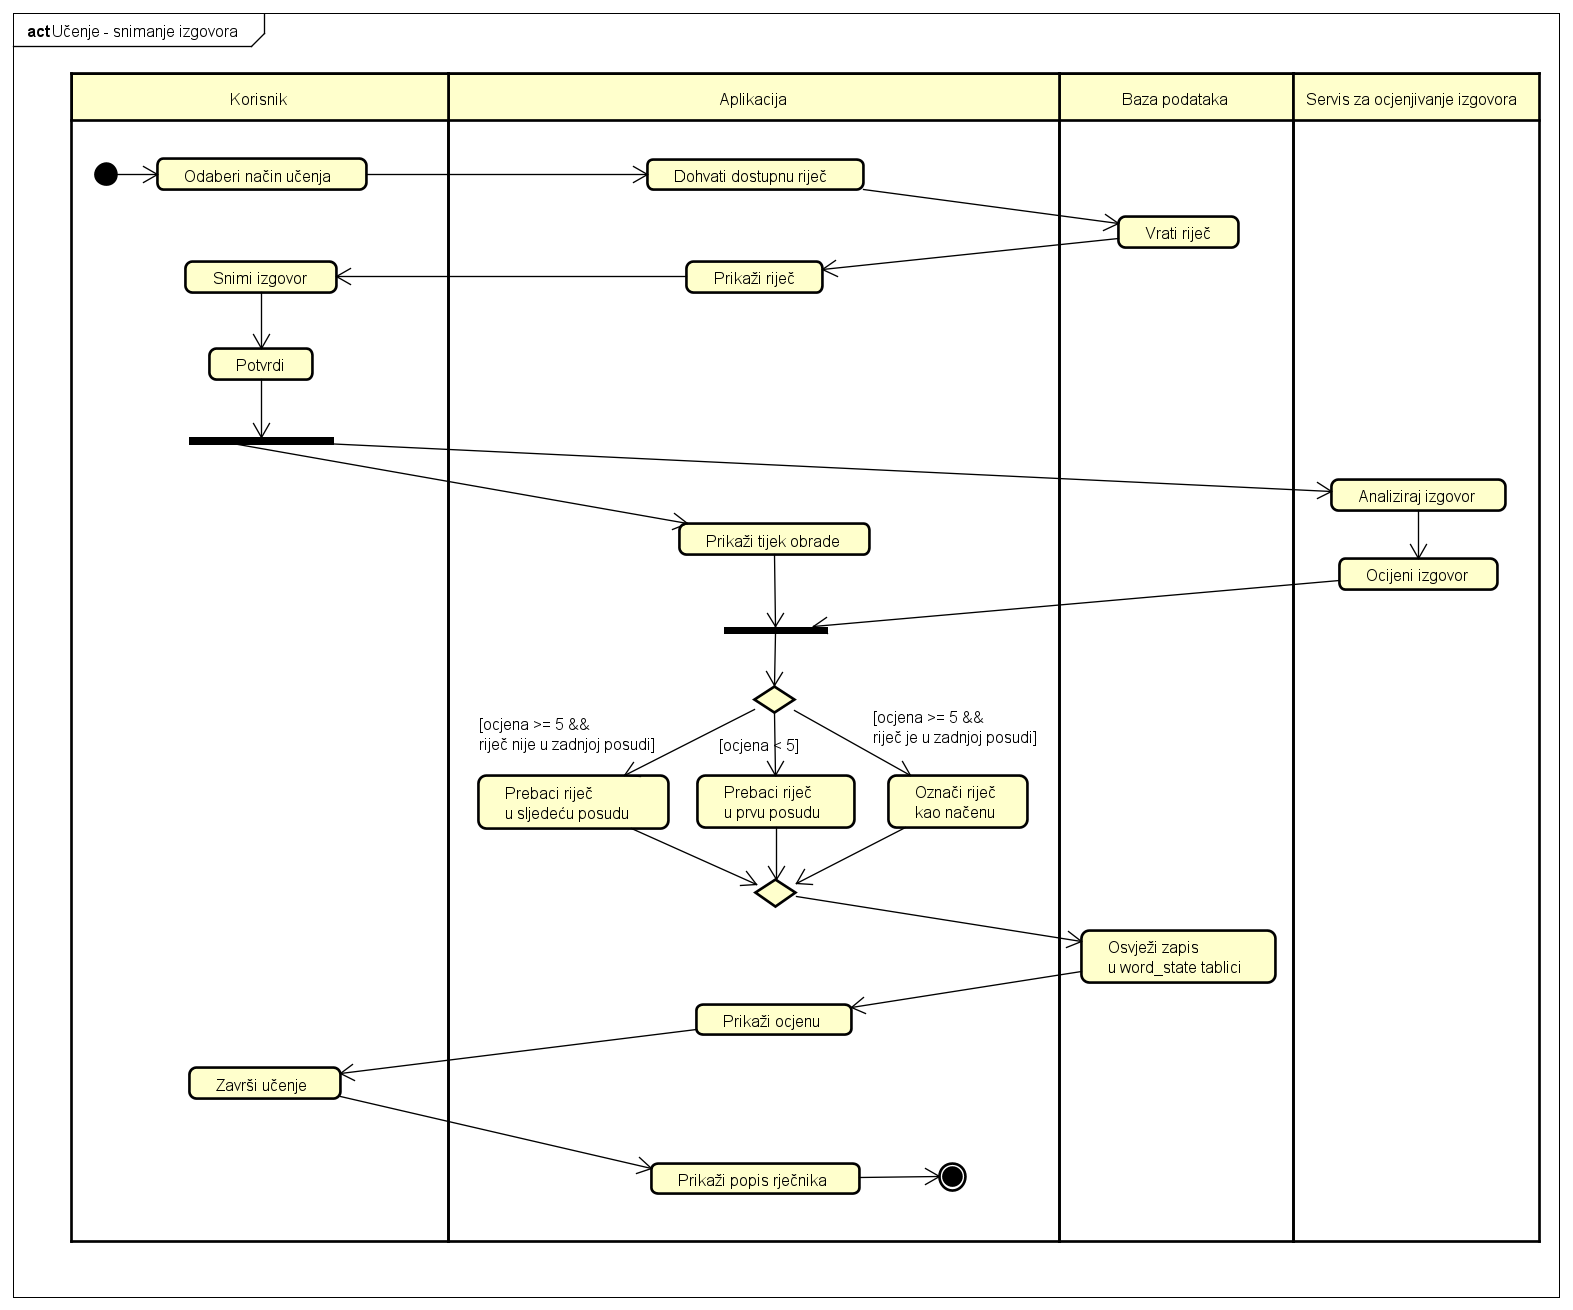
\includegraphics[scale=0.4]{dijagrami/aktivnosti.png}
	\centering
	\caption{Dijagram aktivnosti za učenje sa snimanjem izgovora}
	\label{fig:aktivnosti-izgovor}
\end{figure}


			\eject
		\section{Dijagram komponenti}

\begin{figure}[htp]
	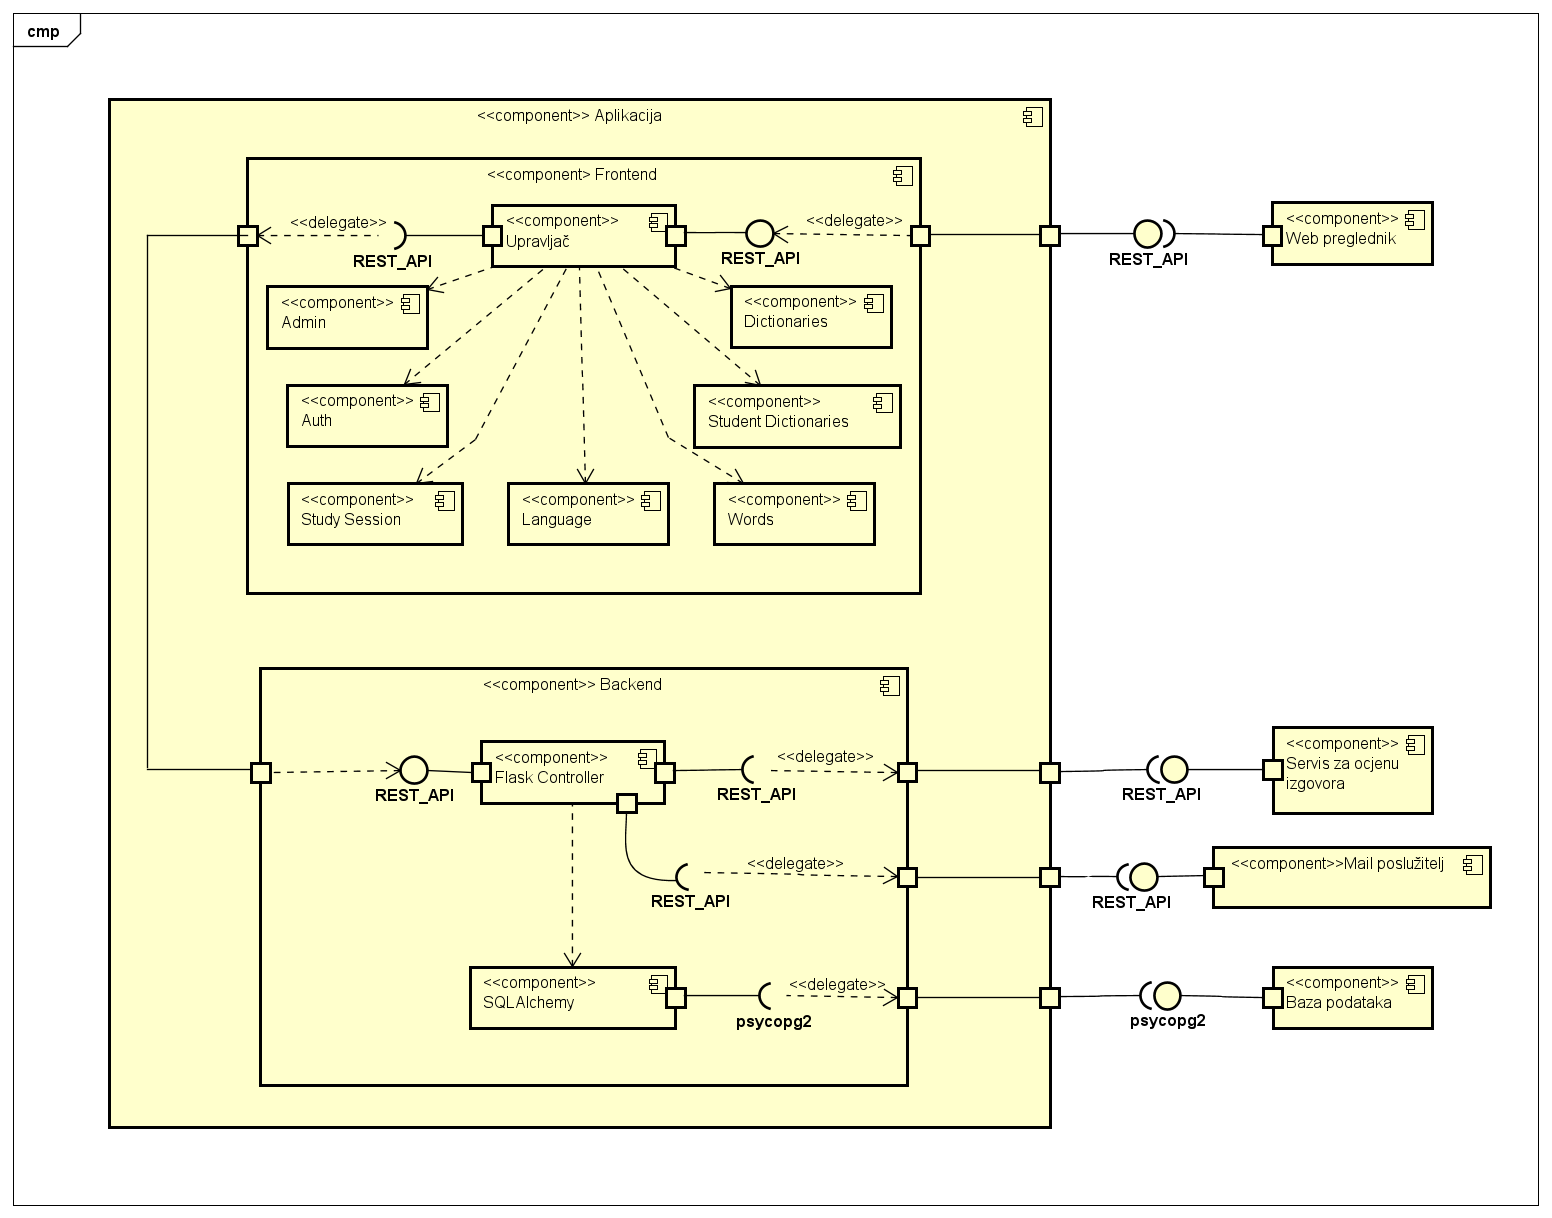
\includegraphics[scale=0.4]{dijagrami/ComponentDiagram0.png}
	\centering
	\caption{Dijagram komponenti}
\end{figure}